\chapter{System Design}

\section{List of Symbols}


\begin{table}[htbp]
    \centering
    \begin{tabular}{l l}
        \hline
        \textbf{Symbol/Formula} & \textbf{Description} \\
        \hline
        \((KS)_E\) & Origin of the coordinate system on the inclined plane \\
        \( _{(E)}\vec{p}(t) \) & 3D vector of the total motion in plane \((KS)_E\)\\
        \(_{(E)}\vec{p_B} (t) \) & 3D vector of pure motion in plane \((KS)_E\) \\
        \(_{(E)}\vec{p_0}\) & 3D start vector. User input (gap width)\\
        \(z(t)\) & Motion equation of the robot trajectory \\
        \(\hat{z}\) & User input for the lifting height\\
        \(\omega\) & Angular frequency \\
        \(f\) & User input for the frequency \\
        \(W\) & Physical work \\
        \(F\) & Physical force \\
        \(P\) & Physical power \\
        \hline
    \end{tabular}
    \caption{List of Symbols and Formulas}
\end{table}

\section{Motion Profile of the Paddle Mixer}

\begin{figure}[h]
    \centering
    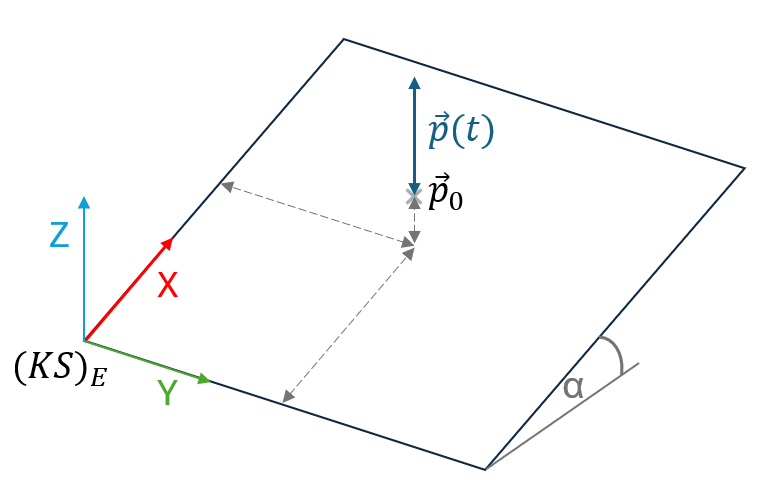
\includegraphics[width=0.8\textwidth]{bilder/KS_E-Koordinatensystem_Ebene.png}
    \caption[Visualization of the Coordinate System on the Inclined Plane]{Visualization of the Coordinate System on the Inclined Plane (own illustration)}\label{fig:VisualizationCoordinateSystemInclinedPlane}
\end{figure}

\noindent The following describes the three parameters for a reproducible description of the paddle movement in all three directions of motion. Here, \( _{(E)}\vec{p}(t) \) represents the total movement in the coordinate system \((KS)_E\). \(_{(E)}\vec{p_B} (t) \) describes the variable position starting from \(_{(E)}\vec{p_0}\).\\

\textbf{General:}

\begin{equation}
    \begin{aligned}
        _{(E)}\vec{p}(t) &= _{(E)}\vec{p_B}(t) + _{(E)}\vec{p_0}\\
        \text{with}\\
        _{(E)}\vec{p}_B(t) &= _{(E)}\left(x_B(t), y_B(t), z_B(t)\right)\\
        _{(E)}\vec{p_0} &= _{(E)}\left(x_0, y_0, z_0\right)
    \end{aligned}
    \label{eq:generalMovement}
\end{equation}

\autoref{eq:generalMovement} is independent of the initiated type and direction of movement. Any possible types of movement can be represented in \(\vec{p}_B(t)\).\\

The calculation based on a sinusoidal movement along the Z-axis follows:

\begin{equation}
    \begin{aligned}
        _{(E)}\vec{p}_{0} &= (x_{0}, y_{0}, z_{0})\\
        _{(E)}\vec{p}(t) &= (x, y, z(t)) + \vec{p}_{0}  
    \end{aligned} 
\end{equation}

\( z(t) \) is defined by:

\begin{equation}
    z(t) = -\hat{z}(\cos(\omega t)-1)  \quad \text{with} \quad \hat{z} = \frac{h}{2}
\end{equation}

and \( \omega = 2 \pi f = \frac{2 \pi}{T} \).

For example, at \( t = 0 \):

\begin{equation}
    z(0) = -\hat{z}(1-1) = 0
\end{equation}

Example at \( t = \frac{1}{4}T \):

\begin{equation}
    \begin{aligned}
        z\left(\frac{1}{4}T\right) &= -\hat{z}\left(\cos\left(\frac{2\pi T}{T \cdot 4}\right) - 1\right) \\
        &= -\hat{z}\left(\cos\left(\frac{\pi}{2}\right) - 1\right) \\
        &= -\hat{z}(0 - 1) = \hat{z} = \frac{1}{2} h
    \end{aligned}
\end{equation}

And at \( t = \frac{1}{2}T \):

\begin{equation}
    \begin{aligned}
        z\left(\frac{1}{2}T\right) &= -\hat{z}\left(\cos\left(\frac{2\pi T}{T \cdot 2}\right) - 1\right) \\
        &= -\hat{z}\left(\cos(\pi) - 1\right) \\
        &= -\hat{z}(-1 - 1) = 2\hat{z} = h
    \end{aligned}
\end{equation}

where \( _{(E)}\vec{p(t)} \) represents the movement of the paddle center and \( _{(E)}\vec{p}_{0} \) represents the center on the single-use bag.

\begin{figure}[h]
    \centering
    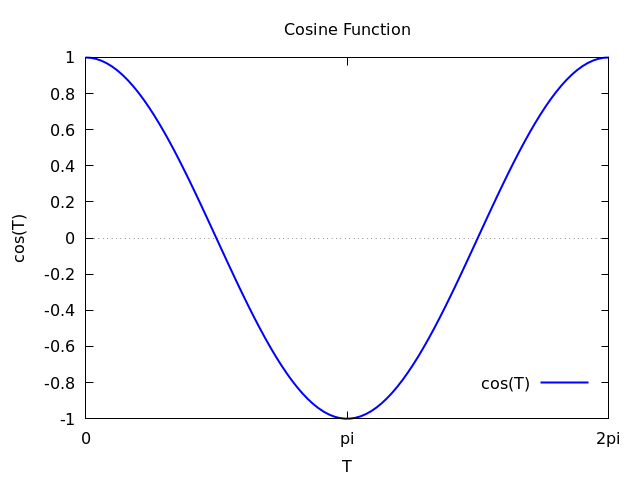
\includegraphics[width=0.8\textwidth]{bilder/cosine-plot.png}
    \caption[Cosine Function]{Classical cosine function (\( cos(t) \)) (own illustration)}\label{fig:CosineFunction}
\end{figure}
\FloatBarrier

\begin{figure}[h]
    \centering
    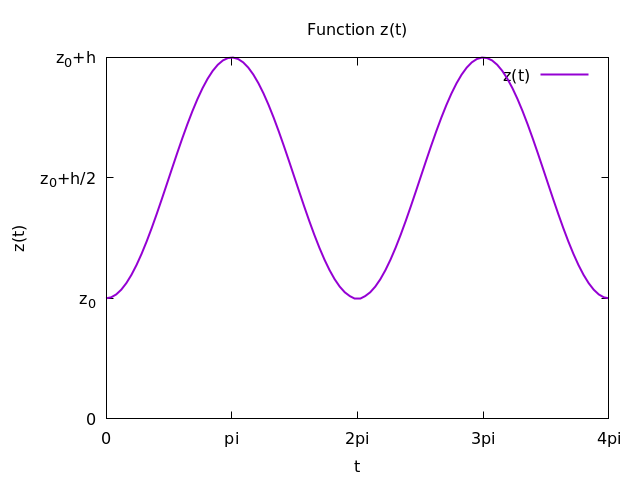
\includegraphics[width=0.8\textwidth]{bilder/cosine-plot_real.png}
    \caption[Representation of Paddle Movement Using the Cosine Function]{Representation of the paddle movement in the Z-direction using the cosine function \( z(t) = -\hat{z}(\cos(\omega t)-1) \) (own illustration)}\label{fig:PaddleMovementCosine}
\end{figure}
\FloatBarrier

Example sinusoidal movement in \( _{(E)}\) Z-direction:
\begin{equation}
    \begin{aligned}
        x &= x_B + x_0\\
        y &= y_B + y_0\\
        z(t) &= \hat{z}\left( 1 - \cos(\omega t) \right) +z_0\\
        \text{with}\\
        &\hat{z} = 2h\\
        &\omega = 2\pi f
    \end{aligned}
\end{equation}

\section{Definition of Power Input for the Mixing Process}

Generally, it holds:

\begin{equation}
    W = \int_{t_1}^{t_2} \vec{F}(\vec{s(t)})\cdot d \vec{s}
\end{equation}

\noindent If the force direction matches the motion direction and both vectors point in the same direction, it holds:

\begin{equation}
    W = F \cdot s \text{   and   } P = \frac{W}{dt}
\end{equation}

\noindent In our case, the force \(F_z\) points in the direction of motion \(z\), but it is not constant. Therefore, it holds:

\begin{equation}
    \begin{aligned}
        W = \int_{t_1}^{t_2} F_z (z(t))\cdot dz\\
        W = \int_{t_1}^{t_2} F_z (t)\cdot dz
    \end{aligned}
\end{equation}

The relationship between force and distance is
